\section{Графическое изображение матожидания критерия}
Вычислим матожидание от имеющегося векторного критерия для игрока П
$F(X, Y) = \big(\frac{Y\sqrt{X}}{2};\frac{\sqrt{1-X}}{Y}\big)$, где $X$ и $Y$ - случайные величины, причём
\[
\begin{cases}
P(X=0)=1-q \\
P(X=1)=q \\
\end{cases}
\begin{cases}
P(Y=1)=1-p \\
P(Y=2)=p \\
\end{cases}
\]

В таком случае имеем:
\begin{equation}
\E_{x} [F(x,y)]=\big(\frac{yq}{2};\frac{1-q}{y}\big)
\end{equation}
\begin{equation}
\E_{xy} [F(x,y)]=\big(\frac{q(1+p)}{2};\frac{(1-q)(2-p)}{2}\big)
\end{equation}

Рассмотрим это как множество точек на плоскости $X,Y$ зависящие от двух параметров $(p,q)\in[0,1]^2$
\[
\begin{cases}
y=\frac{q(1+p)}{2} \\
x=\frac{(1-q)(2-p)}{2}  
\end{cases}
\Rightarrow
\begin{cases}
q=\frac{2x}{1+p} \\
y=(1-\frac{2x}{1+p})\frac{2-p}{2}=\frac{(1+p-2x)(2-p)}{2(1+p)}
\end{cases}
\]

Найдём максимальные значения, которые может принимать $y(x, p)$ при фиксированном $x$:
$$
\frac{\partial{y(x,p)}}{\partial{p}}=\frac{3x}{(p+1)^2} - \frac{1}{2}=0 
\Rightarrow
p_0=\sqrt{6x} - 1
$$
Поскольку область определения $p_0\in[0, 1]$, и 
$$
p_0 = 1 \Rightarrow x=\frac{2}{3} \textsl{ и }
p_0 = 0 \Rightarrow x=\frac{1}{6}
$$
 
$$y_{max}(x) = 
\begin{cases}
\max(y(x, 0), y(x, 1), y(x, p_0)), & x\in[\frac{1}{6}, \frac{2}{3}] \\
\max(y(x, 0), y(x, 1)), & x\in[0, \frac{1}{6}] \cap [\frac{2}{3}, 1]
\end{cases}
$$

учитывая, что 
$$y(x, 0) = 1 - 2x $$
$$y(x, 1) = \frac{1-x}{2}$$ 
$$y(x,p_0) = \frac{(\sqrt{6x} - 2x)(3-\sqrt{6x})}{2\sqrt{6x}}$$

$$y_{min}(x)=
\begin{cases}
\frac{1-x}{2}, &x\in[0,\frac{1}{3}] \\
1-2x, &x\in(\frac{1}{3},1]
\end{cases}
\quad
y_{max}(x)=
\begin{cases}
1-2x, &x\in[0,\frac{1}{6}] \\
\frac{(\sqrt{6x} - 2x)(3-\sqrt{6x})}{2\sqrt{6x}}, &x\in(\frac{1}{6},\frac{2}{3}]\\
\frac{1-x}{2}, &x\in(\frac{2}{3},1]
\end{cases}
$$

В предыдущем пункте мы установили что любая пара $(p^{*}, q^{*}) \in [0, 1]^{2}$ является оптимальной. Теперь для всех
оптимальных стратегий т.е. пар $(p^{*}, q^{*}) \in [0, 1]^{2}$ изобразим на графике значения матожидания векторного критерия в этой
точке.
\begin{center}
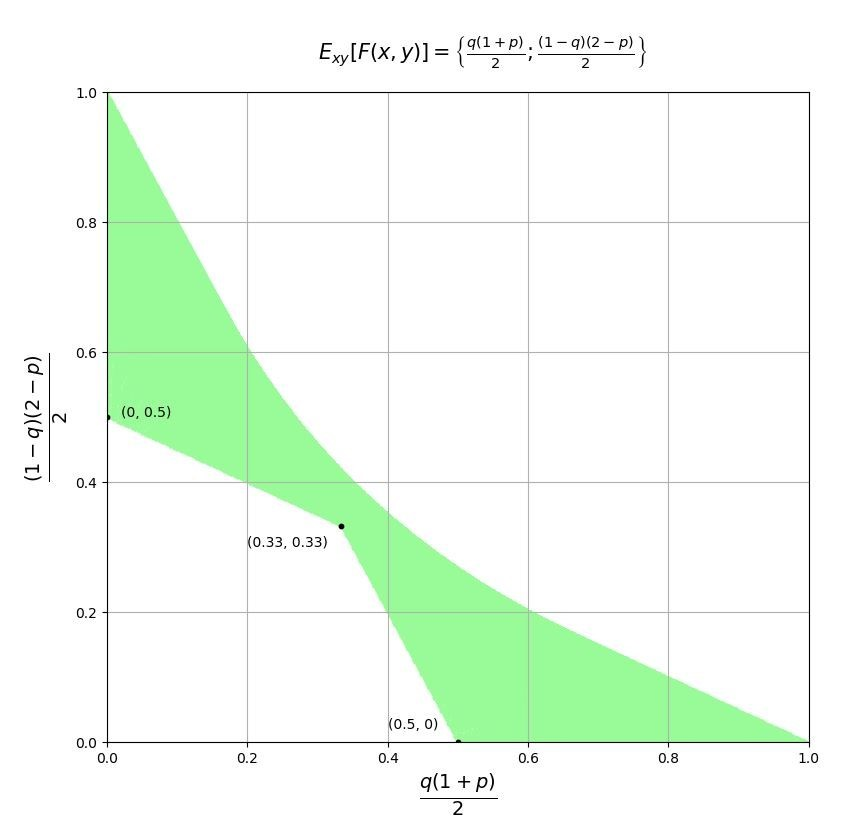
\includegraphics[scale=0.8]{part_2/graf_1_2}
\end{center}

